\documentclass[fleqn,10pt]{wlscirep}
\usepackage[utf8]{inputenc}
\usepackage[T1]{fontenc}

\title{Homework two report}

\author[1,*]{Y.Q. Yang}


\begin{abstract}    
According to the result obtained from the following analysis, transcription activator B plays a more important role in cancer.

\end{abstract}
\begin{document}

\flushbottom
\maketitle

\thispagestyle{empty}

\section*{Results}

\subsection*{Quality Control}

To check if there exists any microarry chips that perform abnormally, I first briefly visualized the distribution of expression level for each chip in Relative Log Expression Level(REL) with the package \textit{Oligo}. \cite{csdn.net} It is revealed that the total expression level among these chips are approximately the same.  Consequently, I can make sure that all microarry data are reliable and can be applied to subsequent analysis.

\begin{figure}[ht]
    \centering
    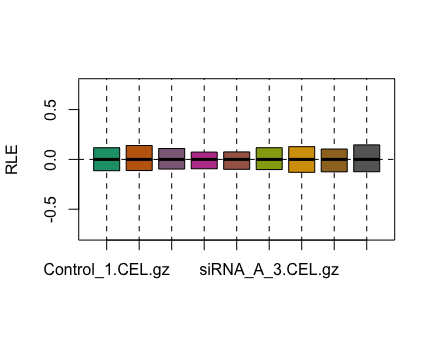
\includegraphics[width=15cm,height=10cm]{RLE.png}
    \caption{Relative Log Expression Level(REL) for each chip}
    \label{fig:stream}
    \end{figure}

\subsubsection*{Differential Expression Gene Analysis}

Rawdata retrieved from chips are read in with the package \textit{Affy}, and are pretreated using \textit{rma} algorithm, which are proved to have a better performance in enhancing the signal from Perfect Match(PM) probes \cite{jianshu.com}. 

By respectively comparing the data retrieved from transcription-activator-A-knocked out(abbreviated as sample A below) and transcription-activator-B-knocked out(abbreviated as sample B below) samples with data from control samples, a Differential Expression Gene Analysis has been performed. Result shows that more genes are differentially expressed in samples treated with siRNA B, The threshold of differntial expression is determined by $abs(logFC) > 1.5$ and $adj.P.value < 0.05$ so as to remove as much false positive results as possible.  The result are drawn as volcanoplots listed below.
After figuring out the number of significantly expressed genes respectively in sample A and B, I found that sample B contains dramitically higher number of differential expressed genes.

\begin{table}[ht]
    \centering
    \begin{tabular}{|l|l|l|}
    \hline
    group & sample A & sample B \\
    \hline
    number & 7 & 264 \\
    \hline
    \end{tabular}
    \caption{\label{tab:example}number of significantly expressed genes }
    \end{table}

\begin{figure}[h]
    \begin{minipage}[t]{0.45\linewidth}
    \centering
    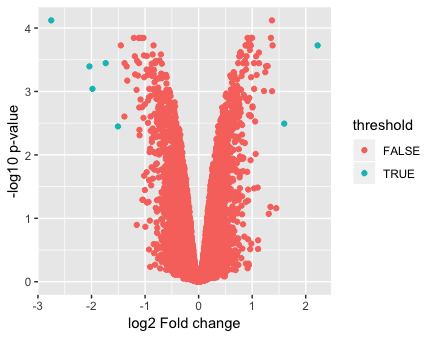
\includegraphics[width=7cm,height=6.5cm]{sA.png}
    \caption{volcanoplot of sample A}
    \end{minipage}
    \begin{minipage}[t]{0.45\linewidth}        %图片占用一行宽度的45%
    \hspace{2mm}
    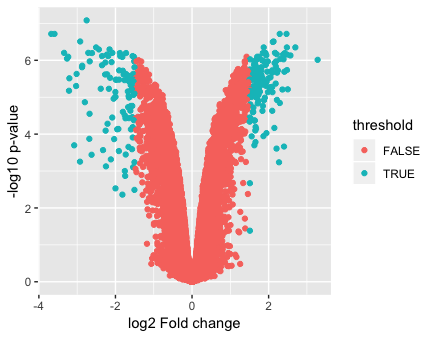
\includegraphics[width=7cm,height=6.5cm]{sB.png}
    \caption{volcanoplot of sample B}
    \end{minipage}
\end{figure}

\subsection*{Probable Impact of Transcription Activator B on Cancer}
After clustering the differential expressed genes obtained in the previous step by Genetic Oncology(GO) Analysis and Kegg Analysis, I found that the transcription activator B plays a role in cancer probably through interfering cell cycle 

\subsubsection{Genetic Oncology(GO) Analysis}

\subsubsection{Kegg Analysis}

\subsubsection{GSEA Analysis}

\subsection*{A/B Gene Hypothesis}

\begin{itemize}
\item First item
\item Second item
\end{itemize}


 
Topical subheadings are allowed.

\section*{Discussion}

The Discussion should be succinct and must not contain subheadings.

\section*{Methods}

Topical subheadings are allowed. Authors must ensure that their Methods section includes adequate experimental and characterization data necessary for others in the field to reproduce their work.

\bibliography{sample}

\noindent LaTeX formats citations and references automatically using the bibliography records in your .bib file, which you can edit via the project menu. Use the cite command for an inline citation, e.g.  \cite{Hao:gidmaps:2014}.

For data citations of datasets uploaded to e.g. \emph{figshare}, please use the \verb|howpublished| option in the bib entry to specify the platform and the link, as in the \verb|Hao:gidmaps:2014| example in the sample bibliography file.

\section*{Acknowledgements (not compulsory)}

Acknowledgements should be brief, and should not include thanks to anonymous referees and editors, or effusive comments. Grant or contribution numbers may be acknowledged.

\section*{Author contributions statement}

Must include all authors, identified by initials, for example:
A.A. conceived the experiment(s),  A.A. and B.A. conducted the experiment(s), C.A. and D.A. analysed the results.  All authors reviewed the manuscript. 

\section*{Additional information}

To include, in this order: \textbf{Accession codes} (where applicable); \textbf{Competing interests} (mandatory statement). 

The corresponding author is responsible for submitting a \href{http://www.nature.com/srep/policies/index.html#competing}{competing interests statement} on behalf of all authors of the paper. This statement must be included in the submitted article file.





Figures and tables can be referenced in LaTeX using the ref command, e.g. Figure \ref{fig:stream} and Table \ref{tab:example}.

\end{document}